
\section*{Теоретическое введение}
\subsection*{Магнитное поле в веществе}

Магнитное поле на уровне атомов может резко изменяться в пространстве и времени. Такую физическую величину практически невозможно измерить, поэтому рассматриваются физически бесконечно малые объёмы вещества. Такой объём вещества достаточно мал, чтобы его размерами можно было пренебречь, но содержит достаточно большое количество частиц, чтобы магнитное микрополе можно было усреднить.

Для описания усредненного магнитного поля вводится вектор \textit{намагниченности} $\vec{M}$, который равен суммарному магнитному дипольному моменту единицы объёма. Тогда средняя индукция магнитного поля в данном бесконечно малом объёме равна:
$$
\vec{B} = \mu_0 (\vec{H} + \vec{M}),
$$
$\mu_0 = 4 \pi \cdot 10^{-7}$ -- магнитная постоянная.

В простейшем случае намагниченность сонаправлена с вектором напряженности внешнего магнитного поля:
$$
\vec{M} = \chi \vec{H}
$$
Коэффициент $\chi$ называется магнитной восприимчивостью среды.

\subsection*{Доменная структура ферромагнетиков}

В отличие от диа- и парамагнетиков ферромагнетики сильно намагничиваются даже в слабых полях. Как и у парамагнетиков, атомы ферромагнетиков имеют собственный магнитный момент. Но в отсутствие внешнего магнитного поля магнитные моменты образуют упорядоченные структуры --- \textit{домены}, в которых они ориентированы практически в одном направлении.

\begin{wrapfigure}{l}{0.42\linewidth}
	\vspace{-10pt}
	\centering
	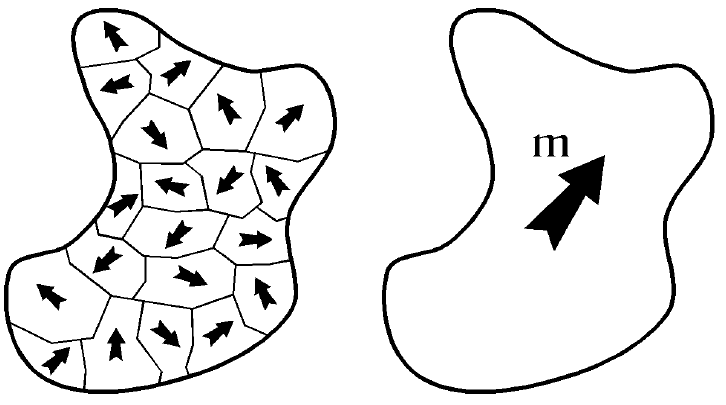
\includegraphics[width=0.70\linewidth]{../res/domens.png}
	\caption{Доменная структура ферромагнетика в слабом (слева) и сильном (справа) внешнем магнитном поле.}
	\label{img:domen}
\end{wrapfigure}

Образование доменов в ферромагнетиках не может быть обусловлено магнитным взаимодействием дипольных моментов соседних атомов, так как энергия такого взаимодействия мала по сравнению с тепловой. Единственными силами, которые могут упорядочить магнитные моменты, являются квантовые электростатические силы взаимодействия электронов. <<Энергетически выгодной>> оказывается следующая структура ферромагнетика:

\begin{enumerate}
	\item Соседние магнитные моменты атомов ориентируются в одном направлении, образуя домены, так как энергия электростатического отталкивания электронов в этом случае минимальна. Такое явление называется \textit{обменным взаимодействием}.
	
	\item Домены имеют конечный размер, а соседние ориентированы противоположно. Если рассмотреть ферромагнетик, состоящий из одного большого домена, то окажется, что энергия доменного взаимодействия мала, но в этом случае ферромагнетик создает сильное магнитное поле, которое обладает большой энергией. При дроблении ферромагнетика на домены, энергия магнитного поля уменьшается, а энергия взаимодействия соседних доменов увеличивается. Дробление прекращается, когда сумма энергий магнитного поля и доменного взаимодействия достигает минимума.
\end{enumerate}

\subsection*{Теория ферромагнетизма Вейса}

Впервые количественная теория, описывающая ферромагнетизм была разработана французским физиком Вейсом в 1907 году. Согласно этой теории, магнитные моменты соседних атомов взаимодействуют между собой с силами, зависящими от угла между магнитными моментами. Эти силы стремятся ориентировать магнитные моменты в одном направлении, что приводит к образованию доменов. Также предполагается, что эффективное магнитное поле в веществе равно сумме внешнего магнитного поля $\vec{H}$ и микрополя $\vec{H_{микр}}$. Микрополе создаётся магнитными моментами соседних атомов и пропорционально намагниченности вещества $M$.
$$
\vec{M} = \chi \vec{H_{эфф}}
$$
$$
\vec{H_{эфф}} = \vec{H} + \beta \vec{M}
$$
где $\beta$ - некоторая константа, называемая постоянной Вейса.

Эмпирическая теория Вейса имеет физическое обоснование на основе квантовой механики. Если при рассмотрении закона Кулона в классической механике ввести добавочные силы взаимодействия, то результат получится таким же, как если применять законы квантовой механики. Эти силы называются \textit{обменными} и нужны для согласования классической и квантовой теорий. Они являются короткодействующими и при определенных условиях, связанных с внутренним строением вещества стремятся установить спины электронов соседних атомов параллельно друг другу, что и объясняет образование доменов в ферромагнетиках. Согласно эксперименту, обменное взаимодействие может быть с достаточной точностью учтено введением некоторого эквивалентного молекулярного поля $\beta \vec{M}$.

\subsection*{Гистерезис}

\begin{wrapfigure}{r}{0.42\linewidth}
	\vspace{-10pt}
	\centering
	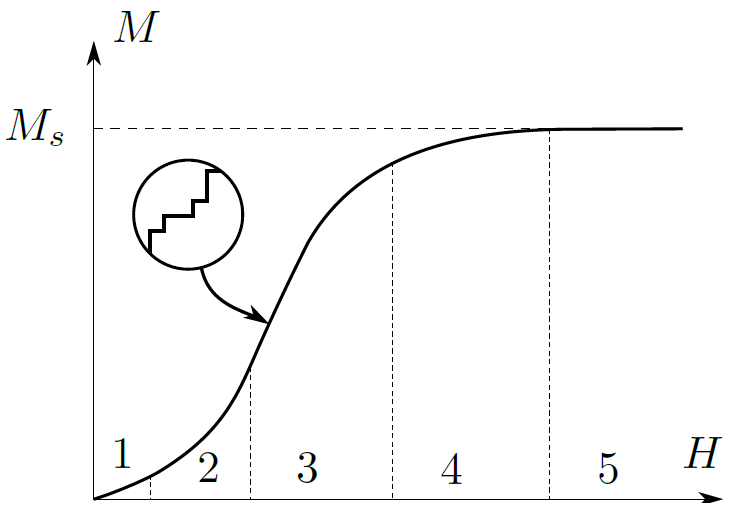
\includegraphics[width=0.90\linewidth]{../res/magnetization curve.png}
	\caption{Начальная кривая намагниченности ферромагнетика.}
	\label{img:domen}
\end{wrapfigure}

Зависимость намагниченности $\vec{M}$ ферромагнетика от напряженности внешнего магнитного поля является не линейной.

Рассмотрим \textit{начальную кривую намагниченности} $\vec{M}(\vec{H})$. Эту кривую разделяют на пять участков:

\textit{Область обратимого намагничивания 1}. В этой области намагниченность пропорциональна внешнему магнитному полю $\vec{M} = \chi \vec{H}$. Домены, которые ориентированы вдоль поля, увеличиваются в размере за счёт переориентировки магнитных моментов соседних атомов. Такой процесс называется упругим смещением границ и является обратимым.

\textit{Область Рэлея 2}. Зависимость намагниченности от внешнего поля является квадратичной. В этой области смещение границ является обратимым, но зависимость становится квадратичной.

\textit{Область наибольший проницаемостей 3}. В этой области происходят необратимые смещения стенок доменов и наблюдается наибольший рост намагниченности. Из-за наличия особенностей структуры вещества (дефекты кристаллической решетки, примеси), существуют силы, которые препятствуют движению границ доменов. Поэтому домену нужно накопить достаточную энергию для преодоления этих сил, то есть движение стенок доменов носит скачкообразный характер (\textit{скачки Баркгаузена}). В следствие скачкообразного изменения границ доменов, скачками меняется и намагниченность.

\textit{Область приближения к насыщению 4}. Движение стенок доменов в этой области прекращается. Энергетически выгодно становится поворачивать магнитные моменты оставшихся, неориентированных по полю доменов.

\textit{Область насыщения 5}. В этой области все домены ориентированы по полю, а дальнейшее увеличение внешнего магнитного поля не меняет намагниченность вещества.

При медленном уменьшении напряженности магнитного поля из состояния насыщения, из-за наличия взаимодействия между доменами и особенностей структуры вещества домены, домены будут продолжать ориентированы в одном направлении. Только после достаточного уменьшения внешнего поля, часть доменов изменит свою ориентацию. Из этого видно, что кривая намагниченности не будет совпадать с начальной. Такое явление, когда состояние вещества зависит от истории изменений, называется \textit{гистерезисом}. Рассмотрим предельную петлю гистерезиса.

\begin{wrapfigure}{r}{0.42\linewidth}
	\vspace{-10pt}
	\centering
	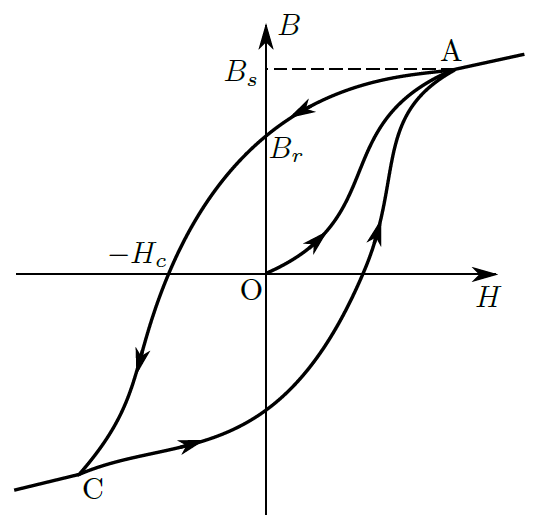
\includegraphics[width=0.90\linewidth]{../res/hysteresis.png}
	\caption{Начальная кривая намагниченности ферромагнетика.}
	\label{img:domen}
\end{wrapfigure}

В точках $A$ и $C$ достигается насыщение, соответствующее значение индукции магнитного поля $B_s$ называется \textit{индукцией насыщения}. Кривая $OA$ является начальной кривой намагничивания. При медленном уменьшении магнитного поля из состояния насыщения, кривая намагниченности проходит выше начальной кривой. При нулевом внешнем магнитном поле, намагниченность ферромагнетика не обращается в ноль, соответствующее этому состоянию значение $B_r$ называется \textit{остаточной индукцией}. Чтобы намагниченность ферромагнетика стала равна нулю, нужно создать магнитное поле $H_c$, направленное противоположно начальному, которое называется \textit{коэрцитивным}. Цикл $A-C-A$ называется предельной петлей гистерезиса. Площадь цикла в координатах $H-B$ есть энергия, необратимо выделяющаяся в единице объема вещества за один цикл:
$$
\Delta \omega = \oint_S H \,dB
$$

\subsection*{Тороид}

\begin{wrapfigure}{r}{0.3\textwidth}
	\vspace{-30pt}
	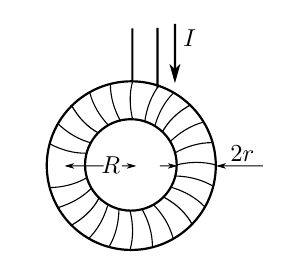
\includegraphics[width=\linewidth]{../res/tor.png}
	\caption{Тороид с намагничевающей обмоткой}
	\label{img:tor}
	\vspace{30pt}
\end{wrapfigure}

Напряженность магнитного поля $H$ в катушке, равномерно намотанной на тороид, определяется из теоремы о циркуляции:

$$ \oint (\vec{H}, \vec{dl}) = I_{out}. $$

Тогда для тороида получаем:

\begin{equation}
	H = \frac{N_0 I}{2 \pi R}
	\label{eq:H_tor}
\end{equation}

\subsection*{Интегрирующая ячейка}

\begin{wrapfigure}{r}{0.4\textwidth}
	\vspace{-10pt}
	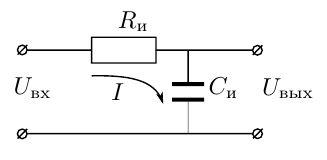
\includegraphics[width=\linewidth]{../res/integr.png}
	\caption{Интегрирующая ячейка}
	\label{img:integr}
	\vspace{10pt}
\end{wrapfigure}

Рассмотрим катушку с числом витков $N$, намотанную на образец площадью $S$, индукция магнитного поля $B$ однородна. Тогда из закона электромагнитной индукции:

$$ B = \frac{1}{SN} \int \mathcal{E} dt. $$

В этом случае для измерения индукции магнитного поля $B$ можно воспользоваться интегрирующей цепочкой \figref{img:integr}. В случае, если ток $I$ будет почти постоянным, выполнится следующее соотношение:

$$ U_{\text{вых}} = \frac{q}{C_{\text{и}}} = \frac{1}{C_{\text{и}}} \int_{0}^{t} U_{\text{вх}} dt $$

Для постоянства тока требуется, чтобы $R_{\text{вх}} \ll R_{\text{и}} \ll R_{\text{вых}}$, а также $R_{\text{и}}$ такое, что за $\frac{1}{\nu_{\text{вх}}}$ почти все напряжение было на $R_{\text{и}}$.

Подставляя второе соотношение в первое, получим:
\begin{equation}
	B = \frac{\tau_{\text{и}}}{SN} U_{\text{вых}}
	\label{eq:B_circuit}
\end{equation}

\section*{Методика эксперимента}


\begin{wrapfigure}{r}{0.5\textwidth}
	\vspace{-10pt}
	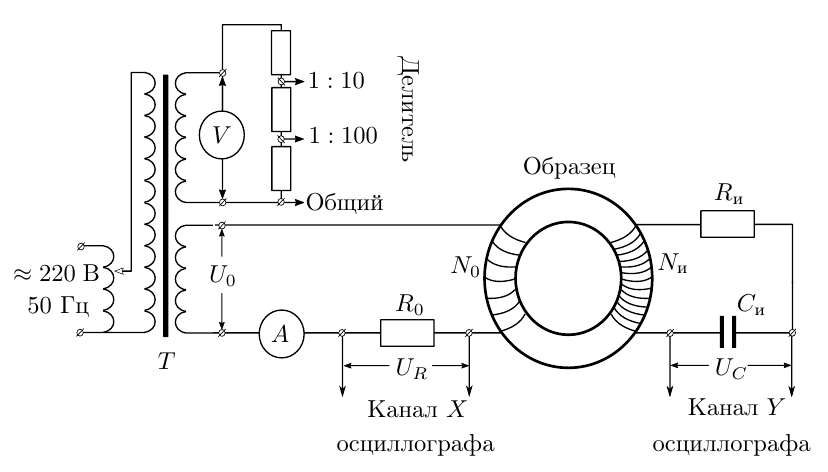
\includegraphics[width=\linewidth]{../res/scheme.png}
	\caption{Схема установки}
	\label{img:scheme}
	\end{wrapfigure}

В эксперименте используется установка, приведенная на рис. \ref{img:scheme}. Напряжение из сети ($U = 220$ В, $\nu = 50$ Гц) с помощью трансформаторного блока конвертируется в $U_0 = 6.3$ В, $\nu_0 = 50$ Гц. Напряжение $U_0$ подается на первичную катушку образца. Значение напряженности магнитного поля $H$ в образце связано с током через первичную катушку $I$ (см. \ref{eq:H_tor}), поэтому для измерения $I$ $X$-канал осциллографа подключен к резистору $R_0$: $U_X = I_0 R_0$. Ко вторичной обмотке подключена интегрирующая ячейка, позволяющая определить значение поля $B$ в образце. В соответствии с \ref{eq:B_circuit} $Y$-канал осциллографа подключен к конденсатору $C_{\text{и}}$.

Для определения количественных параметров полученной на экране осциллографа кривой требуется определить масштабы изображения. Чтобы определить масштабы $K_X$, $K_Y$ требуется провести калибровку. Для этого используется амперметр $A$.

% TODO: Изменерие напряженности и индукции магнитного поля в образце.

% TODO: RC-цепь.